\subsection{(Anti-)(hyper-)nuclei production} 
\subsubsection{Thermal production and nucleon coalescence models}
\label{sec:producionmodels}

The production of light (hyper-)nuclei and their anti-matter counterparts is modeled within the two scenarios of thermal-statistical hadronisation and nucleon coalescence.
In the thermal-statistical approach \cite{Andronic:2010qu, Andronic:2017}, particles are produced from a fireball in thermal and kinetic equilibrium with temperatures of the order of $T_{chem} \approx$ 156 MeV that are near the temperature of the QCD phase transition boundary, as predicted by lQCD calculations \cite{Bazavov:2014pvz,Bellwied:2013cta}.
The yields of the produced objects depend on the chemical freeze-out temperature $T_{chem}$ (when inelastic collisions cease) and the mass $m$ of the object, and approximately scale as d$N$/d$y \propto \exp(-m/T_{chem})$.  
Thermal-statistical models have been successful in describing light-flavour particle production across a wide range of energies in nucleus-nucleus collisions \cite{Andronic:2017, Acharya:2017bso}.  
Due to their large mass, light (anti-)(hyper-)nuclei are particularly sensitive to $T_{chem}$ and since they are not affected by feed-down from higher mass states, the measurement of their production constitutes a precision test for the thermal model.  

In the coalescence scenario, composite objects are formed at kinetic freeze-out by coalescence of nucleons that are close in configuration and momentum space \cite{Butler:1963, Kapusta:1980, Bergstrom:1979gpv, Sato:1981ez, Nagle:1996vp, Scheibl:1998tk}. Calculations of the coalescence probability based on a density matrix approach \cite{Scheibl:1998tk} require the knowledge of the nucleus wave function and identify the volume of the particle source with the homogeneity volume that can be extracted via Hanbury-Brown-Twiss interferometry \cite{Wiedemann:1999qn}. 

%The quantum-mechanical nature of the process is encoded in an average quantum-mechanical correction factor that depends on the size of the nucleus, on the homogeneity volume of the particle source and, via the latter, on the transverse momentum of the coalescing nucleons.
\begin{figure}[t]
\begin{center}
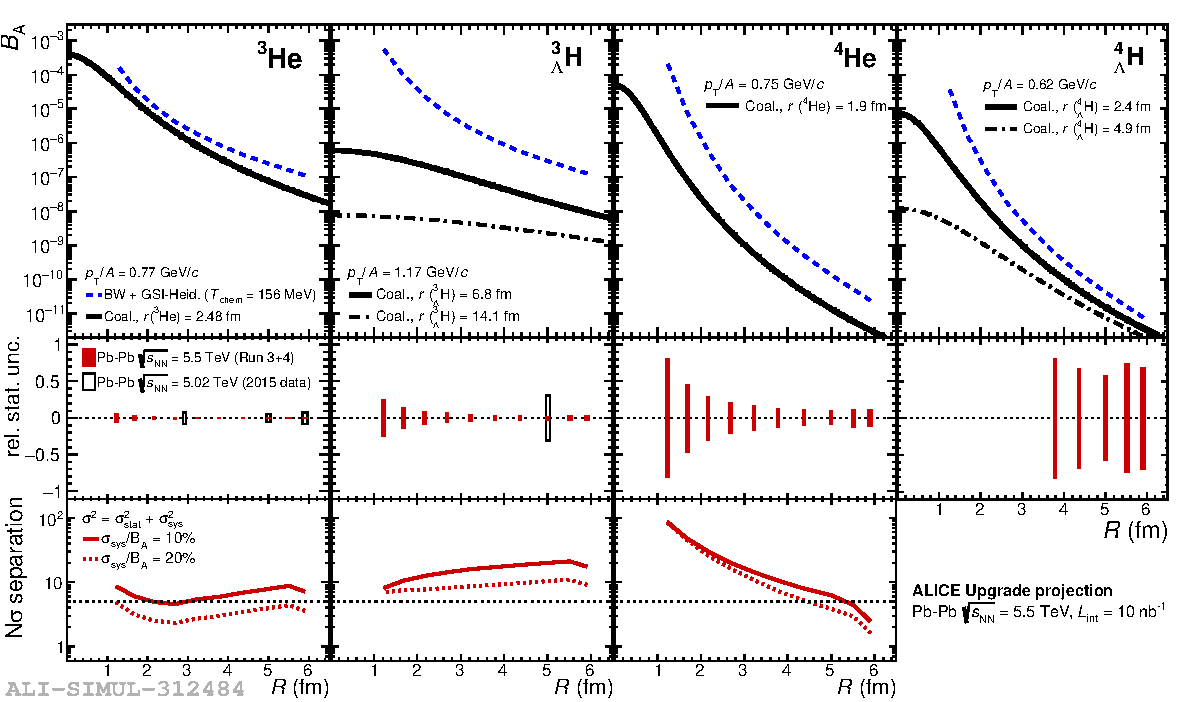
\includegraphics[width=\textwidth]{\main/lightflavour/figs/2018-10-23-2018-10-23-BAmodels_pseudoUnc.pdf}
\end{center}
\caption{
Top: comparison of predictions for the coalescence parameters for (hyper-)nuclei with $A = 3, 4$ from the Blast-Wave + GSI-Heidelberg thermal statistical model and coalescence (see legend for the considered rms radius) as a function of the system radius, $R$. See \cite{Bellini:2018epz} for full details on the models. Middle: projection of the relative statistical uncertainty achievable with a Pb--Pb integrated luminosity of \textit{L}$_{int} = 10 \mathrm{nb}^{-1}$ and the upgraded ALICE detector (in red) compared to the relative statistical uncertainty of the Run 2 measurements (in black). Bottom: expected significance in the discrimination between the two models, assuming 10$\%$ and 20$\%$ systematic uncertainty in addition to the expected statistical uncertainty.}
\label{fig:BAmodels}
\end{figure}

While there are several theory groups working on the calculation of the expected coalescence \cite{Scheibl:1998tk, Cho:2017dcy, Zhang:2018euf, Bazak:2018hgl, Zhao:2018lyf} and thermal production rates \cite{Andronic:2010qu, Wheaton:2004qb, Petran:2013dva}, predictions reported in Fig.~\ref{fig:BAmodels} rely on the study presented in~\cite{Bellini:2018epz}, which contrasts the two production scenarios. 
In order to distinguish them, a measurement of the coalescence parameter for (anti-)(hyper-)nuclei that differ by mass, spin and size (rms of the wave function) as a function of source volume (or radius) is proposed. The size of the source is sampled by means of multiplicity- and centrality-differential measurements.
The particle with the strongest sensitivity to the production mechanism appears to be the hypertriton (a bound state of a proton, a neutron and a $\Lambda$ hyperon), with its wide rms radius of about 10 fm, for which the coalescence and the thermal model predictions differ up to about two orders of magnitude as a function of the source radius. 
In particular, \hyp~is predicted by coalescence to be suppressed by about a factor 100 with respect to \hethree~in pp collisions. 
While the hypertriton seems to be largely suppressed with respect to \hethree, the \hypfour\ is predicted to have only a slightly lower coalescence probability with respect to \hefour. This motivates a systematic measurement of nuclei and hyper-nuclei with $A=4$ as a function of centrality and from small to large systems.

\subsubsection{Light (anti-)(hyper-)nuclei production with the LHC Run 3 and 4}
\label{sec:hyper}
Measurements of (anti-)(hyper-)nuclei and exotic QCD bound states require large event samples collected with a minimum-bias trigger, as well as high tracking precision for the separation of secondary vertices and charged-hadron (light nucleus) identification. The upgraded ALICE detector after LS2 \cite{Abelevetal:2014dna, ALICE:2014qrd,alice-up-trg,Buncic:2015ari} fulfills these requirements, thus confirming the strong potential of ALICE and its data-taking program for these studies.

The signal yield of (hyper-)nuclei (d,  \hethree, \hefour, \hyp, \hypfour, \hyphefour) and their antiparticles have been estimated to be measured with ALICE in Pb--Pb collisions at the LHC Run 3 and 4. 
Expected yields and significance for central (0--10\%) Pb--Pb collisions are reported in Fig.~\ref{fig:yieldrun34} for anti-particles as a function of the minimum-bias integrated luminosity. The same amount of particles and anti-particles is expected. 
All the predictions have been done in the 2--10~\gmom\ \pT\ interval and for the nominal magnetic field of the ALICE detector (B~=~0.5~T). The $\pT = 2~\gmom$ value represents the lower limit where nuclei with $A~\geq~3$ can be reconstructed without ambiguities in ALICE. 
During Run 3, ALICE plans to take data with a central-barrel low-field configuration (B~=~0.2~T) and to collect data in Pb--Pb collisions up to $L_{int} = 3~\mathrm{nb}^{-1}$. 
In this configuration, it will be possible to extend the low-\pT\ limit for \mbox{(anti-)nuclei} identification down to 1~\gmom, increasing the expected number of detectable light \mbox{(anti-)(hyper-)nuclei.} 
In Fig.~\ref{fig:yieldrun34}, the bands indicate the uncertainty on the expected yield 
(significance) associated with different model predictions:
the central line is obtained using the statistical-thermal model~\cite{Andronic:2010qu} with $T~=~156$~MeV, the upper line is the yield (significance) expected from the thermal model with $T~=~158$~MeV,  and the lower one the expectation from coalescence (see Sec.~\ref{sec:producionmodels}). 
The black box in the right corner of each panel is a multiplicative factor which represents the potential improvements with the upgraded Inner Tracking System (ITS).  The arrow represents the luminosity expected at the end of LHC Run 2. 
%This The predicted yields at \sqrtsNN = 5.5~TeV (the actual energy after LS2) are very close to those 
%at \sqrtsNN = 2.76~TeV~\cite{Andronic:2010qu}. 

\begin{figure}%[hbpt]
\begin{center}
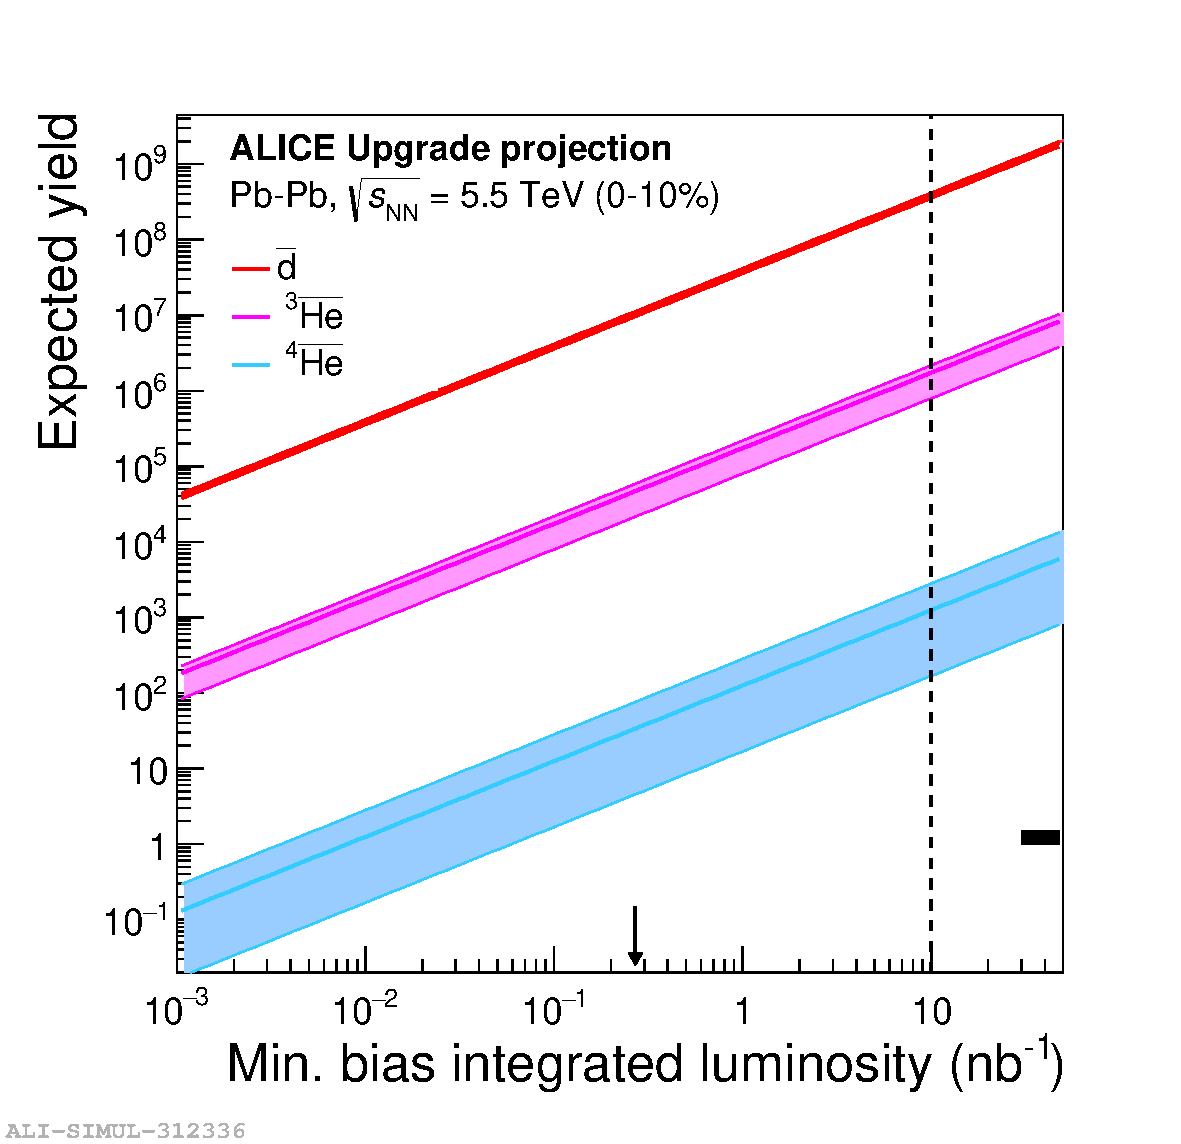
\includegraphics[width=0.49\textwidth]{\main/lightflavour/figs/2018-10-23-2018-10-23-nuclei_projection_10nb-1-presentITS.pdf}
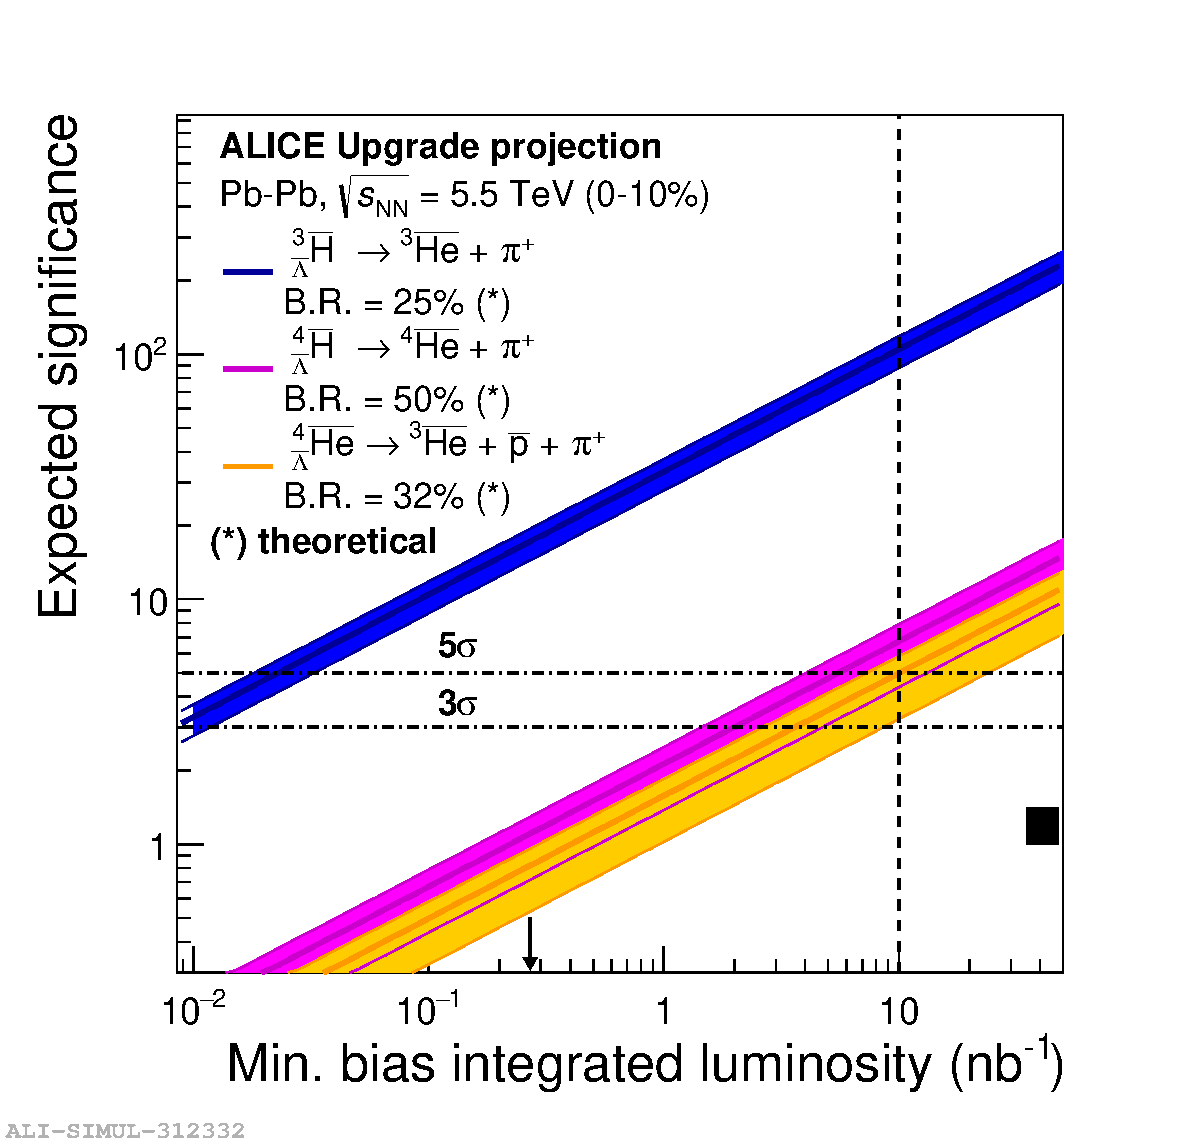
\includegraphics[width=0.49\textwidth]{\main/lightflavour/figs/2018-10-23-2018-10-19-hypernuclei_significance_10nb-1-presentITS.pdf}
\end{center}
\caption{Left: Expected yield of anti-nuclei in 0--10$\%$ central Pb--Pb collisions with ALICE as a function of the minimum bias luminosity in the $2 <\pt< 10~\gmom$ interval. 
Right: Projected significance of anti-hyper-nuclei measurements in central Pb--Pb collisions in Run 3 and 4 with ALICE as a function of the integrated minimum-bias luminosity. In both panels, the arrow and the vertical line represent the minimum bias Pb--Pb luminosity at the end of Run 2 and Run 4, respectively. The bands represents the uncertainty on model prediction for the yield (see text for details) and the black box in the right corner denotes a multiplicative factor representing the possible improvements related to use of the upgraded ALICE ITS.}
\label{fig:yieldrun34}
\end{figure}

The expected yield per unit of rapidity at mid-rapidity in the $2<\pt<10$~\gmom\ 
interval for \antid, \antihethree\ and \antihefour~(and the corresponding nuclei) 
are reported in left panel of Fig.~\ref{fig:yieldrun34}.
The large statistics that will be collected for anti-nuclei with $A = 3$  will allow 
to test the Charge Symmetry Breaking (CSB) in the anti-nuclei sector due to the differences in the 
up and down quark masses and due to electromagnetic effects \cite{Miller:1990ky}. 
The differences in $A = 3$ systems are extensions of the neutron-proton difference. 
Although the mass difference for the lightest ``mirror pair'' with $A = 3$ (\tritium,\hethree), 
is well known (at the level of O(eV)~\cite{Audi:2002rp}), no measurements have been performed in the anti-matter sector. 
The large data sample that will be collected will lead to the first precise measurements of the mass of light anti-nuclei with $A=3$ by means of the Time-Of-Flight detector~\cite{Adam:2015pna}.
%
In addition, a measurement of the elliptic flow ($v_2$) of \hethree~and \tritium~(and anti-nuclei) will become feasible with a statistical precision better than 5$\%$ in the 2-10 GeV/$c$ transverse momentum range, in at least eight centrality intervals with ALICE. Elliptic flow measurements for anti-nuclei provide a powerful independent test of coalescence scenarios and an indirect assessment of the neutron flow by comparison of \hethree~and \tritium~results, as already tested with deuterons \cite{Acharya:2017dmc}.

In the right panel of Fig.~\ref{fig:yieldrun34}, the expected significance of anti-hyper-nuclei measurements in central Pb--Pb collisions is reported as a function of the integrated luminosity, for the decay channels reported in the legend. 
Considering the thermal model predictions at $T~=~156$~MeV, the expected significance 
of \antihyp, \antihypfour\ and \antihehypfour\ at the end of Run 4, is 100, 7 and 5, respectively. 
The collected sample will enable very precise measurements of the production of \hyp\ and \antihyp\ and the first ever measurement of their elliptic flow as a function of \pT.
The discovery of \antihypfour\ and \antihehypfour\ will be in reach at the end of Run 4.

In addition, theory calculations for the $\Sigma NN$ system suggest the presence of a near-threshold narrow ($\sim$2~MeV wide) quasi-bound state with isospin 1 and spin 1/2 ~\cite{cite:SigmaTriton-theory}. Among $\Sigma$-hypernuclei, only the $_{\Sigma^0}^{4}\mathrm{He}$ bound state has been observed so far, using the ${^4}\mathrm{He}(K^-,\pi^-)$ reaction \cite{cite:SigmaTriton-data}.
Experimental searches for $\Sigma$-hypertriton bound states will also profit from the Pb--Pb data-taking program of the LHC Run 3 and 4 to exploit the decay
$\sigmahyp (\antisigmahyp) \rightarrow \hyp (\antihyp) + \gamma$, driven by
the electromagnetic decay of 
$\Sigma^{0}(\overline{\Sigma}^{0}) \rightarrow \Lambda(\overline{\Lambda}) + \gamma$.
%When the hyperon is bound inside a nucleus, the electromagnetic decay however is dominated by the conversion reaction $\Sigma^{0} N \rightarrow \Lambda N$, thus the width is expected to broaden substantially. \todo{ change ``reduce'' with broaden !!! em is narrower than strong channel }
%
%with B.R.~=~100$\%$ \todo{Stefano P: Sigma in the nucleus undergoes the strong interaction with nucleons, i.e. the conversion reaction Sigma N -> Lambda N, which is the main decay of a possible sigma-hypernucleus. The conversion reaction width is about 15 MeV but in the hypernucleus dynamics various mechanisms and selections rules are expected to suppress the width substantially (5-10 MeV). Anyway, the main decay channel should be the conversion reaction and not the free decay. Therefore, I would rephrase accordingly.}.
In ALICE, the signal of hypertriton can be reconstructed as discussed in Sec.~\ref{sec:hyper}, while the soft photon can be identified by exploiting the conversion into electron pairs in the detector material of the ITS and Time Projection Chamber ($X/X_o = 11.4 \%$) or the Transition Radiation Detector ($X/X_o = 24.7 \%$), or detected in the Photon Spectrometer.
Given the expected performance for hypertriton detection in ALICE (see Fig. \ref{fig:yieldrun34}, see \cite{Borissov:2015ura} for $\Sigma^{0}$ reconstruction), about 10$^3$ $\Sigma$-hypernuclei candidates may be detected in 0-10$\%$ central Pb--Pb collisions corresponding to a minimum bias target luminosity of 10 $\mathrm{nb}^{-1}$. 
The expected significance for \sigmahyp, obtained by downscaling the one for hypertriton by the 1$\%$ efficiency of the photon detection, is of the order of few units. 

The validity of the coalescence picture as opposed to thermal production will be tested with multi-differential measurements of the coalescence parameters ($B_A$) for (hyper-)nuclei with $A=3$ and $A=4$. 
With \textit{L}$_{int}~=~10~\mathrm{nb}^{-1}$, $B_A$ for \hethree, \hyp~and \hefour~can be measured in ALICE in up to ten centrality classes with a statistical precision lower than 5$\%$, 10$\%$ and 20$\%$, respectively. 
The expected relative statistical uncertainty on $B_A$ for (hyper-)nuclei with $A>2$ (see central panels of Fig. \ref{fig:BAmodels}) have been estimated by scaling the latest results on deuterons and $\mathrm{^{3}_{\Lambda}H}$ in Pb--Pb collisions respectively, assuming similar background conditions for these measurements. 
In order to estimate the experimental discrimination power between the models (see previous section), relative systematic uncertainties of 10$\%$ and 20$\%$ have been considered, to be compared with a typical 15$\%$ uncertainty of the Run 1 and 2 measurements. 
As seen in the lowest panels of Fig. \ref{fig:BAmodels}, \hyp~ measurements allow for a 10$\sigma$ discrimination between models, even in a pessimistic scenario in all centralities. The discrimination power rises above the 10$\sigma$ level for \hefour~in semi-central and peripheral collisions.  

\subsubsection{The hypertriton lifetime}
The experimental value of the $\Lambda$ separation energy of the \hyp, B$_{\Lambda}$ = 0.13 $\pm$ 0.05 (stat.) $\pm$ 0.04 (syst.) MeV \cite{davis20053}, led to the hypothesis that the lifetime of the hypertriton is equal or only slightly below the free $\Lambda$ lifetime $\tau$($\Lambda$) = 263.2 $\pm$ 0.2 ps \cite{pdg:2017}.
Three different experimental techniques have been used to tackle this question: photographic emulsion, He bubble chambers and counter experiments. The average for the emulsion experiments is 203$^{+40}_{-31}$ ps \cite{agnello:2016}, for the He bubble chambers is 193$^{+15}_{-13}$ ps \cite{agnello:2016} and the combination of both visualizing techniques is 193$^{+14}_{-13}$ ps \cite{agnello:2016}. The counter techniques is used in heavy-ion experiments and the most recent results, 181 $^{+54}_{-39} \pm$ 33 ps and 142 $^{+24}_{-21} \pm$ 29 ps, have been obtained by the ALICE \cite{PhysLettB.754.360} and STAR \cite{PhysRevC.97.054909} experiments respectively. This technique is currently the one with the highest precision (14-16$\%$) and the weighted average of heavy-ion experiments results is 185$^{+28}_{-23}$ ps \cite{agnello:2016}.
However, the few existing theoretical calculations head in the direction of the hypothesis mentioned at the beginning of this section. 
The first theoretical determination of $\tau$(\hyp) (Dalitz and Rayet, \cite{NuovCim.A46}) ranged from 239.3-255.5 ps. More recent calculations from Congleton \cite{jphysg.18.339} and Kamada \cite{Phys.Rev.C57} estimated a value of 232 ps and 256 ps, respectively. The deviation of the experimental results from the theoretical calculations and the free $\Lambda$ lifetime, larger than 2$\sigma$, represents the ``hypertriton lifetime puzzle''.
 
With the expected Pb--Pb integrated luminosity at the LHC Run 3 and 4, the statistical uncertainty on the lifetime will be reduced down to 1$\%$. 
%\todo{Stefano P: there are two values, you must specify what they refer to (hypertrion and anti-hypertriton? Run4 and Run3?)}
In parallel, a reduction of the systematic uncertainty ($\sim$ 10$\%$ in most recent ALICE measurements), will be achieved with the upgraded 
%\todo{bd: before detectors names have been spelled out capital} 
ALICE ITS, that will allow for a reduction of the uncertainty due to tracking and material budget. 
In addition, a better understanding of the corrections for the absorption in the material will be crucial. 

\subsubsection{Exotic QCD bound states}

At the LHC energies, potentially existing 
%\todo{bd: To find something carrying colour would be even more exotic, I would remove the word} 
QCD bound states that have more complex structures such as pentaquarks, tetraquarks, hadron molecules or dibaryon states could be produced.
In particular, the possibility to detect and measure f$_{0}$(980), N(1875), $N\Xi$, $N\Omega$ and $N\Lambda_c$ in heavy-ion collisions with the unprecedented statistics of the HL-LHC program, has been investigated, considering that the excellent capabilities of the ALICE setup in terms of hadron identification, including topological reconstruction of weak decays, are particularly suited for these studies.

\begin{table}
\centering
\resizebox{\textwidth}{!}{
\begin{tabular}{|c|c|c|c|c|c|c|}
\hline
 & Model & f$_{0}$(980)& N(1875)& N$\Xi$& N$\Omega$  & N$\Lambda_{c}$ \\
\hline
\hline
Structure & & $qq\overline{q}\overline{q}$ or $K\overline{K}$& hadron molecule & dibaryon & dibaryon  & dibaryon \\
 \hline
 &  q-coal. & 5.4 $\times$ 10$^{-2}$ &  - & - & 1.8 $\times$ 10$^{-3}$ & 1.5 $\times$ 10$^{-3}$ \\
 
$\big(\frac{\mathrm{d}N}{\mathrm{d}y}\big)_{th}$ & h-coal. & 3.2 $^{\dagger}$       &  - & - & 1.6 $\times$ 10$^{-3}$ & 5   $\times$ 10$^{-3}$ \\

 & thermal &  10  & 3 $\times$ 10$^{-1}$ & 8.7 $\times$  10$^{-3}$ & 5.7 $\times$  10$^{-3}$ & 4 $\times$  10$^{-3}$ \\
\hline \hline
 Decay channel &
 & $\pi\pi$ / $K\overline{K}$ 
 & $\Sigma^{\ast}$K ($\Sigma^{\ast} \rightarrow \Lambda \pi$)   
 & $\Xi\rightarrow \Lambda \pi$ & $\Omega \rightarrow \Lambda$K  
 & $\Lambda_{c}\rightarrow \pi$Kp + $\Lambda_{c}\rightarrow $K$^0$p
\\

 B.R. ($\%$) & & dominant / seen$^{\dagger}$ & unknown (87) & 99.9 & 67.8 & 6.2 + 1.58 \\
Mass (MeV/$c^{2}$) & & 990 & 1850 -- 1920 & - & - & - \\
Width (MeV/$c^{2}$) & & 10 -- 100 & 120 -- 250 & - & - & - \\
\hline
\hline
					 & q-coal. & 1.8 $\times$ 10$^{8}$ & - & - & 6.2 $\times$ 10$^{4}$ & 1.5 $\times$ 10$^{4}$\\
 $\big(\frac{\mathrm{d}N}{\mathrm{d}y}\big)_{exp}$ & h-coal. & 6.4 $\times$ 10$^{6}$ & - & - & 5.5 $\times$ 10$^{4}$ & 5.1 $\times$ 10$^{4}$ \\
  					& thermal & 3.6 $\times$ 10$^{10}$ & 5.5 $\times$ 10$^{7}$& 6.7 $\times$ 10$^5$ & 1.9 $\times$ 10$^{5}$ & 4.1 $\times$ 10$^{4}$\\

\hline
               & q-coal. & 80 & - & - & - & - \\
$\frac{S}{\sqrt{S+B}}$ & h-coal. & - & - & - & - & - \\
 			   & thermal & 15000 & 40 & - & - & - \\

\hline
\end{tabular}
}
\caption{Properties and yields of exotic states in central Pb--Pb collisions (0--10\%) at $\sqrt{s_{\mathrm{NN}}} = 5.5$~TeV. Theoretical predictions of yields per event, (d$N$/d$y$)$_{th}$, are given in three different scenarios: quark- and hadron-coalescence \cite{Cho:2017dcy}, and thermal model \cite{Andronic:2010qu}. (d$N$/d$y$)$_{exp}$ represents the observable yield at the Pb--Pb target luminosity of 10~nb$^{-1}$, taking into account the branching ratios (B.R.) of the decay channels considered and assuming the ALICE detector performance as in Run 2. For f$_0(980)$ and hadron coalescence $^{\dagger}$, a $K\overline{K}$ state with an assumed BR of 10$^{-3}$ is considered. Masses are from \cite{pdg:2017}.}\label{tab:yield}
\end{table}

The yield per event predicted by quark- and hadron-coalescence models \cite{Cho:2017dcy}, and the statistical-thermal model \cite{Andronic:2017} are reported in Tab.~\ref{tab:yield}.
%\todo{bd: Have these yields been provided by Anton? I guess they are in the ExHIC paper and then they use their own calculation, that is particularily different for charm, where GSI-HD have their own way...} --> Reply: we used values provided by Anton.
The expected yields in ALICE are computed at the target integrated luminosity of 10 $\mathrm{nb}^{-1}$ and assuming the same detector performance as in Run 2. 
The significance (see the formula shown in the last row of Tab.~\ref{tab:yield})
%\todo{bd: formula? as in table?} 
for f$_0$(980) and N(1835) was extracted considering for mass and width the values reported in \cite{pdg:2017} and assuming a combinatorial background in the invariant mass range under study.
%\todo{Stefania B: I would also be more precise about the estimation used for the background. Probably being more quantitative on this point it can help also in the reading/understanding of the table.}. 
The expected background was computed from the expected momentum distribution of the decay products as measured in ALICE in Run 2. In particular their momentum components were extracted randomly according to the measured transverse momentum distribution of each candidate (considered as a probability distribution) and assuming a flat probability in $\phi$ and $\eta$ \footnote{A further factor was introduced if the decay particle is reconstructed via invariant mass, since the candidate may belong also to the background.} The obtained significance is reported in Tab.~\ref{tab:yield} for the most pessimistic scenario, in which production occurs via quark coalescence, and the most optimistic scenario, corresponding to thermal production. 

Measurements of f$_{0}$(980) and N(1875) will be feasible in Runs 3 and 4 will shed light on the highly debated nature of the states (hadrons or hadronic molecules). In particular, the N(1875) can be considered a molecular bound state and at the same time the strange partner of the recently discovered pentaquark P$_{c}$ \cite{He:2017PcPartner}. 
Because the structures of exotic states are related to the fundamental properties of Quantum Chromodynamics (QCD), their observation can provide new insights on the properties of QCD at finite temperature and density, for instance the tetraquark condensation may lead to a second chiral phase transition \cite{Cho:2017dcy}.
Several possible states have been studied and predictions are available on the expected yields at LHC energies \cite{Cho:2017dcy}. Among the possible dibaryon bound states the N$\Omega$, N$\Xi$ and $\Lambda_c$N look promising in terms of detection feasibility. Their detection and single baryon correlations will be useful for hyperon correlation studies,  providing new insights in the baryon-baryon attractive potential as well as upper limits in the formation of such bound states in central heavy-ion collisions.

% \begin{table}[h]
% \centering
% \label{tab:yield}       
% % Give a unique label
% % For LaTeX tables you can use
% \resizebox{\textwidth}{!}{%
% \begin{tabular}{|c|c|c|c|c|c|}
% \hline
% State & f$_{0}$(980)& N(1875)& N$\Xi$& N$\Omega$  & N$\Lambda_{c}$ \\
% \hline
% Structure & qq$\overline{q}\overline{q}$ or KK& hadron molecule & dibaryon & dibaryon  & dibaryon \\
% dN/d$y^{th}_{\mathrm{q-coal/h-coal/thermal}}$ & 5.4 10$^{-2}$ / 3.2 $^{\ast}$ / 10 &  - / - / 3 10$^{-1}$ & - / - / 8.7 10$^{-3}$ & 1.8 10$^{-3}$ / 1.6 10$^{-3}$ / 5.7 10$^{-3}$ & 1.5 10$^{-3}$ / 5 10$^{-3}$ / 4 10$^{-3}$ \\
% %dN/deta h-coal & - & - & - & - & - \\
% %dN/deta thermal & - & - & - & - & - \\

% Decay channel & $\pi\pi$/$K\overline{K}$& $\Sigma^{\ast}$K ($\Sigma^{\ast} \rightarrow \Lambda \pi$)  & 
% $\Xi\rightarrow \Lambda \pi$ & $\Omega \rightarrow \Lambda$K  & 
% $\Lambda_{c}\rightarrow \pi$Kp + 
% $\Lambda_{c}\rightarrow $K$^0$p
% \\
% B.R. ($\%$) & dominant (seen$^{\dagger}$) & unknown (87) & 99.9 & 67.8 & 6.2 + 1.58 \\
% Mass (MeV/$c^{2}$)& 990 & 1850 -- 1920 & - & - & - \\
% Width (MeV/$c^{2}$)& 10 -- 100 & 120 -- 250 & - & - & - \\
% dN/d$y^{obs}_{\mathrm{q-coal/h-coal/thermal}}$  & 1.8 $10^{8}$ / 6.4 $10^{6}$ / 3.6 $10^{10}$ & -/-/5.5 $10^{7}$& -/-/6.7 10$^5$ & 6.2 10$^{4}$ / 5.5 10$^{4}$ / 1.9 10$^{5}$ & 1.5 10$^{4}$ / 5.1 10$^{4}$ / 4.1 10$^{4}$\\
% %dN/deta measured h-coal & - & - & - & - & - \\
% %dN/deta measured thermal & - & - & - & - & - \\
% \small{($S/\sqrt{S+B}$)}$_{\mathrm{q-coal/thermal}}$& 80/ 15000 & 40 & - & - & - \\
% %significance h & - & - & - & - & - \\
% %significance th & - & - & - & - & - \
% \hline
% \end{tabular}
% }
% \caption{Properties and yields of exotic states in central Pb--Pb collisions (0--10\%) at $\sqrt{s_{\mathrm{NN}}} = 5.5$~TeV. Theoretical predictions of yields per event, (d$N$/d$y$)$^{th}$, are given in three different scenarios: quark coalescence, hadron coalescence and thermal model. (d$N$/d$y$)$^{obs}$ represents the observable yield at the Pb--Pb target luminosity of 10~nb$^{-1}$, taking into account the branching ratios (B.R.) of the decay channels considered and assuming the ALICE detector performance as in Run 2. For f$_0(980)$ and hadron coalescence, a $K\overline{K}$ state with an assumed BR of 10$^{-3}$ is considered ($^\dagger$). Masses are from \cite{pdg:2017}.}
% \end{table}



